\documentclass[french]{beamer}
  \usepackage[official]{eurosym}
  \usefonttheme[onlymath]{serif}
  \usetheme{lmac}

\begin{document}
  \title[Module Netfilter de filtrage applicatif]{D�veloppement d'un module Netfilter de filtrage applicatif}
  \author[\textsc{Jacob, Whitbeck, Zanotti}]{St�phane \textsc{Jacob}\\John \textsc{Whitbeck}\\Vincent \textsc{Zanotti}}
  \institute[INF]{
    INF 358\\
    T�L�COM ParisTech
  }
  \date[05/2008]{mai 2008}

% FIRST PAGE
  \begin{frame}
    \titlepage
  \end{frame}

  \section<presentation>[]{}
    \begin{frame}
      \frametitle{Introduction : les enjeux du filtrage applicatif}
    \end{frame}

  \section<presentation>[Principes et risques]{Les principes et les risques du filtrage}
  \begin{frame}
    \frametitle{bl�h ?}
      1) les principes et les risques du filtrage (d�tection correcte du
      protocole, extraction des urls, les attaques de bypass (fragmentation,
      re-ordonnancement, utilisation de /flavor/ non standard du protocole),
      r�sistence aux attaques DoS).
  \end{frame}

  \section<presentation>[NetFilter]{Fonctionnement de NetFilter}
  \begin{frame}
    \frametitle{Architecture G�n�rale}
    \begin{figure}
      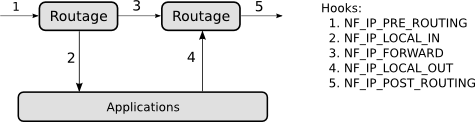
\includegraphics[scale=0.7]{pictures/netfilter.png}
    \end{figure}
  \end{frame}

  \begin{frame}
    \frametitle{Iptables: Principes}
    Fonctions: Regrouper en tables des r�gles de filtrage et de
    modification de paquets IP.

    \begin{center}
      \begin{tabular}{|l|l|}
	\hline
	\textbf{Table} & \textbf{Hooks} \\
	\hline
	filter & INPUT, OUTPUT, FORWARD \\
	\hline
	nat & PREROUTING, POSTROUTING \\
	\hline
	mangle & Toutes \\
	\hline
      \end{tabular}
    \end{center}

  \end{frame}

  \begin{frame}
    \frametitle{Iptables: Exemples}
    \begin{itemize}
    \item Filter: \\ 
      {\tt\scriptsize iptables -t filter -A INPUT -p tcp --dport 80 -j DROP}
    \item Nat: \\
      {\tt\scriptsize iptables -t nat -A POSTROUTING -d ! 192.168.0.0/24 -j
      SNAT --to-source 81.57.230.21}
    \item Mangle: \\
      {\tt\scriptsize iptables -t mangle -A POSTROUTING -p udp --dport 53 -j TOS --set-tos 16}
    \end{itemize}
  \end{frame}

  \begin{frame}
    \frametitle{Conntrack}
    Principe: 
    \begin{itemize}
    \item Regrouper les paquets en flux � partir des triplets (IP
    source, port source, port destination)
    \item Associer � chaque flux un �tat: NEW, ESTABLISHED, RELATED
    \end{itemize}
  \end{frame}

  \begin{frame}
    \frametitle{Extension de NetFilter}
    Plusieurs niveaux:
    \begin{itemize}
    \item Module noyau qui se branche directement sur un hook
    netfilter avec une extension iptables correspondante
    \item Application userspace. On utilise la cible \textrm{NFQUEUE}
    qui d�place un paquet de la m�moire noyau vers une file dans la
    m�moire userspace. Les paquets peuvent alors �tre trait�s par une
    application locale avant d'�tre reinject�s dans NetFilter.
    \end{itemize}
  \end{frame}


  \begin{frame}
    \frametitle{Notre choix}
    Application Userspace car:
    \begin{itemize}
    \item D�veloppement simplifi� et acc�s � des librairies
    puissantes (notamment pour la gestion d'expressions r�guli�res).
    \item Pas de plantage syst�me en cas de plantage de l'application
    \item Minimisation de l'impact d'une faille de s�curit� �ventuelle.
    \end{itemize}
    Mais: 
    \begin{itemize}
    \item Perte de performances due � la copie de la totalit� des
    paquets IP concern�s de la m�moire noyau vers la m�moire userspace
    et vice-versa.
    \end{itemize}
  \end{frame}

  \begin{frame}
    \frametitle{Principe g�n�ral de notre solution}
    \begin{figure}
      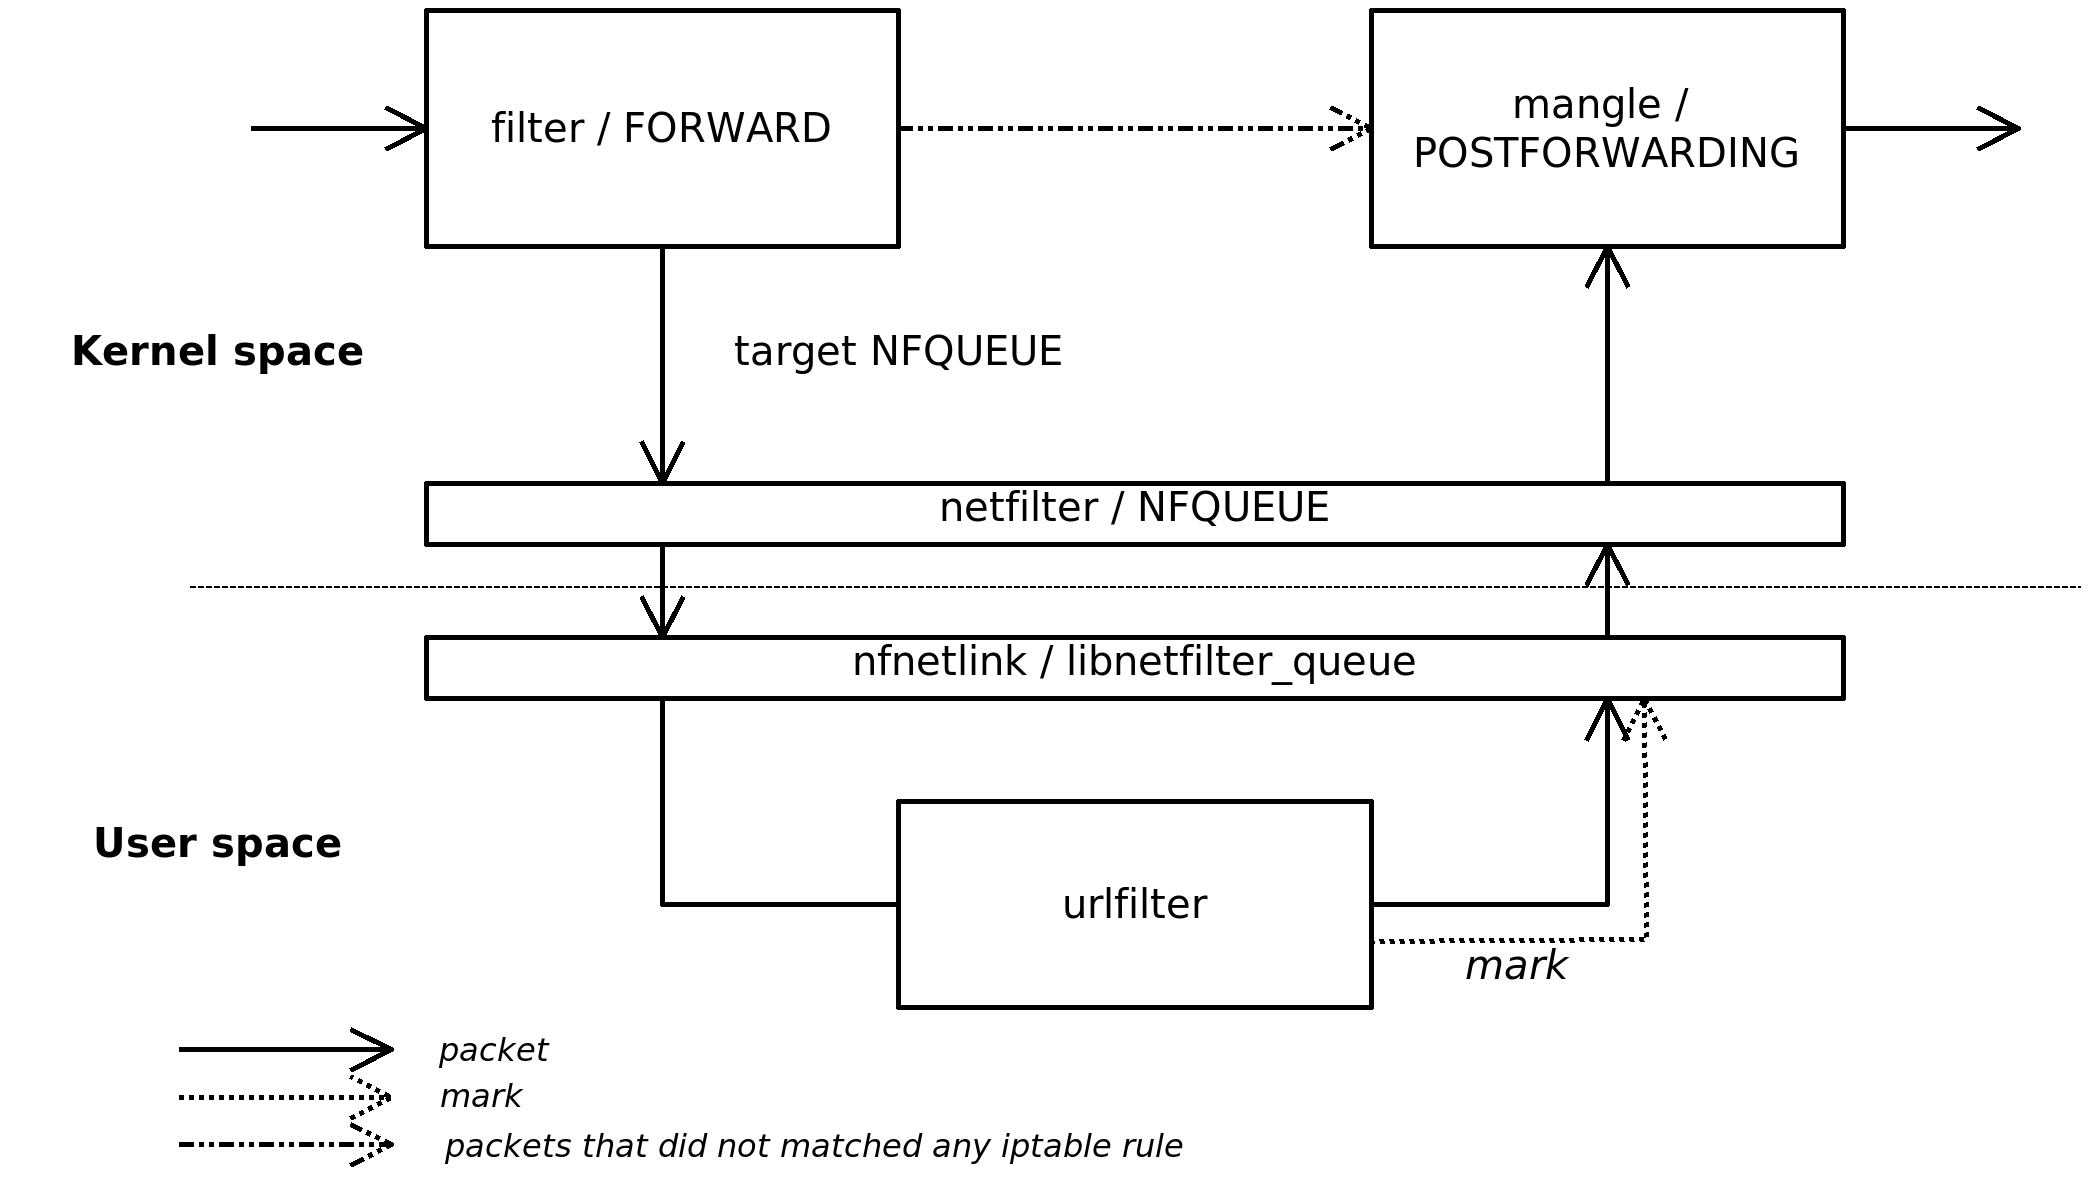
\includegraphics[scale=0.13]{pictures/schema1.png}
    \end{figure}
  \end{frame}

  \section<presentation>[Impl�mentation]{Impl�mentation}
  \begin{frame}
    \frametitle{Organisation du programme}
      Le programme contient :
      \begin{itemize}
        \item un \texttt{README} tr�s complet ;
        \item un r�pertoire base, regroupant plusieurs librairies externes (sous licences compatibles GPLv2) ;
        \item un fichier de configuration ;
        \item \texttt{queue.h/cc}, \texttt{packet.h/cc} et \texttt{conntrack.h/cc} qui r�alisent l'interception des paquets envoy�s �
        \texttt{NFQUEUE} (\texttt{queue.cc}), leur interpr�tation (\texttt{packet.cc}), et leur mise en relation avec un conntrack
        (\texttt{conntrack.cc}) ;
        \item \texttt{classifier.h/cc} qui sert � classer les paquets ;
        \item un fichier de base permettant le lancement des threads, un autre parsant le fichier de configuration et
        initialisant le classifier.
      \end{itemize}
  \end{frame}

  \begin{frame}
    \frametitle{Fonctionnement du logiciel}
      \begin{itemize}
        \item<1-> Regrouper les paquets appartenant � une m�me connexion, gr�ce � l'utilisation de
        \texttt{libnetfilter\_conntrack};
        \item<2-> D�terminer si le contenu de la connexion correspond � un protocole support�;
        \item<3-> Extraire la m�thode et l'url utilis�es par le client des paquets;
        \item<4-> Classifier et remonter l'information au noyau.
      \end{itemize}
  \end{frame}

  \begin{frame}
    \frametitle{Fonctionnement du logiciel}
      \begin{figure}[h]
        \centering
        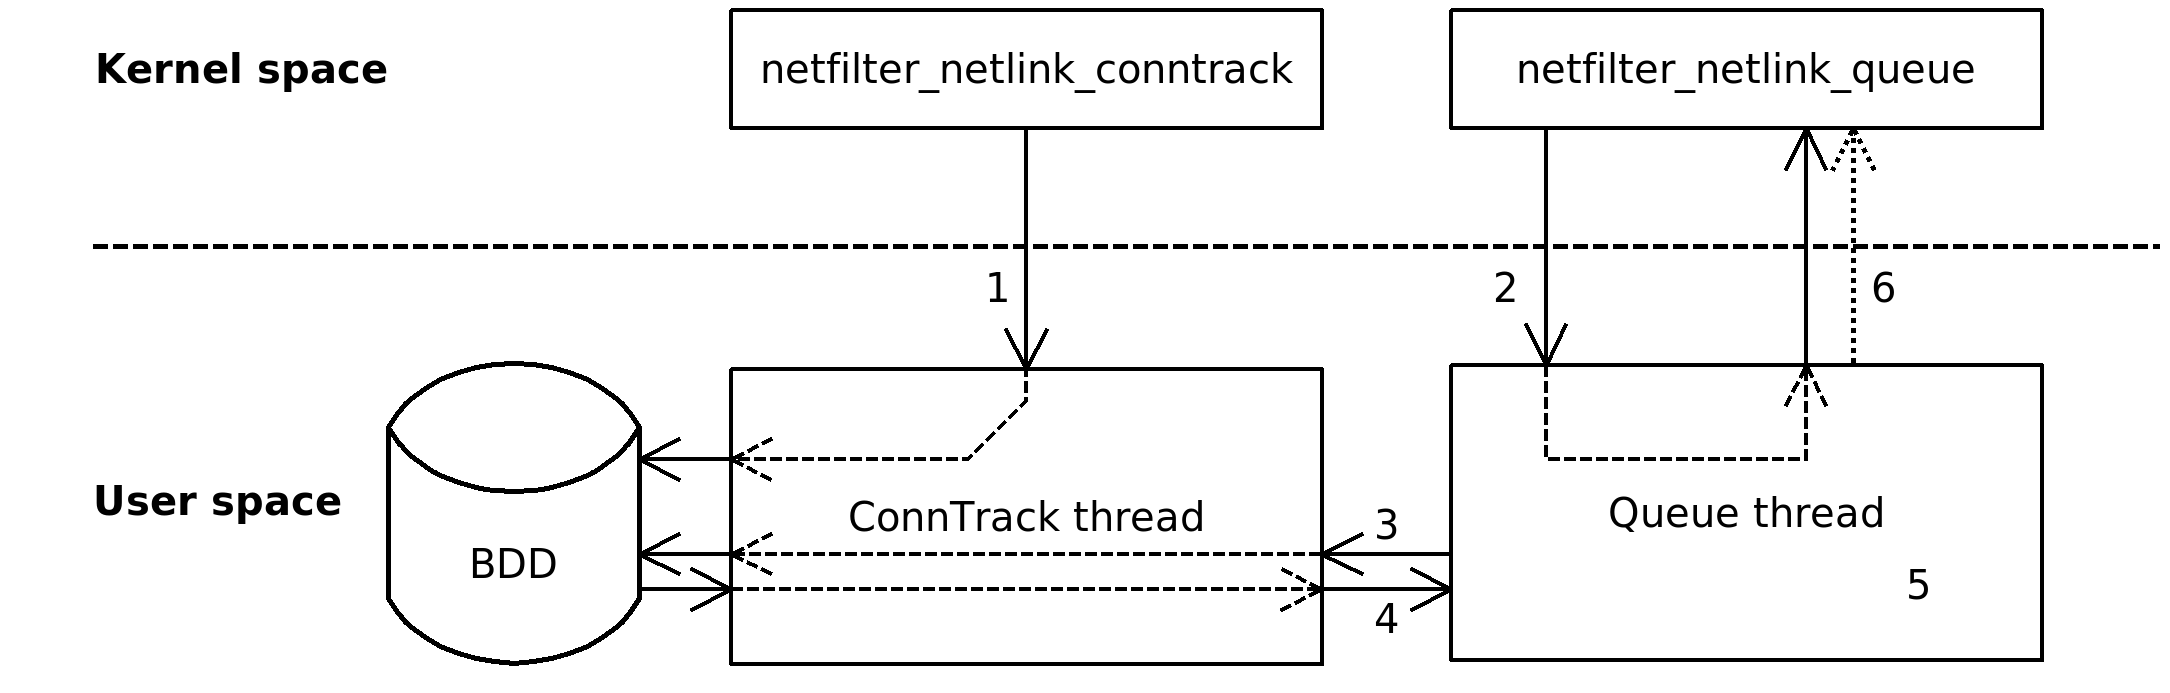
\includegraphics[width=\textwidth]{schema2.png}\\
        \title{Fonctionnement du module}
      \end{figure}
  \end{frame}

  \begin{frame}
    \frametitle{Fonctionnement pratique}
      \begin{itemize}
        \item<1-> Le 1\ier{} thread �coute sur un \texttt{netfilter\_netlink}, re�oit les mises � jour de la table conntrack du
        noyau et maintient une copie locale.
        \item<2-> Le 2\ieme{} thread intercepte les paquets arrivant sur une
        \texttt{NFQUEUE}, les parse, d�termine l'entr�e conntrack et r�cup�re l'objet \og Connection \fg{}
        correspondant, met � jour les deux buffers, puis appelle la m�thode \texttt{update} du classifier avant d'accepter le
        paquet, en le marquant.
        \item<3-> Le classifier surveille les buffers d'une connexion et prend une d�cision.
      \end{itemize}
  \end{frame}

  \begin{frame}
    \frametitle{Fiabilit� et limitation}
      \begin{itemize}
        \item<1-> Le protocole ftp est g�r� correctement.
        \item<2-> Les requ�tes en \emph{Keep-Alive} dans l'http ne sont pas g�r�es.
        \item<3-> L'application r�siste nativement aux attaques de types \emph{Denial of Service}.
      \end{itemize}
  \end{frame}


  \section<presentation>{}
    \begin{frame}
      \begin{center}
        \begin{Huge}
          \textcolor{blue}{Questions ?}
        \end{Huge}
      \end{center}
    \end{frame}
\end{document}
